\section*{Cycle 2 Experiment 2}

\section{\Large{Socket Programming : UDP}}

\subsection{Aim}
\large To implement Client-Server communication using Socket Programming and UDP as transport layer protocol.

\subsection{Theory}
\textbf{UDP (User Datagram Protocol)} is an alternative communications protocol to Transmission Control Protocol (TCP) used primarily for establishing low-latency and loss-tolerating connections between applications on the internet. UDP enables
process-to-process communication. UDP sends messages, called datagrams, and is considered a best-effort mode of communications. It is considered a connectionless protocol because it doesn’t require a virtual circuit to be established before any data
transfer occurs.\\
\\
\textbf{Server \& Client:} Since the UDP is a connectionless protocol, they do not require a connection to get established prior to data transmission or reception. Hence data can be sent between them directly.
\subsection{Algorithm}
\begin{verbatim}
Algorithm for the Client

1 START
2 Create the socket using socket()
3 Configure socket details
4 Connect the socket to server using function connect()
5 Send the message to the server using sendto() 
6 Receive the response from server using recvfrom()
7 Print the response
8 STOP

Algorithm for the Server

1 START
2 Create the UDP socket
3 Configure the socket details
4 Bind the address struct to the socket using bind()
5 Receive from client using recvfrom()
6 Print the received message
7 Send response using sendto()
8 STOP
\end{verbatim}

\subsection{Program \& Output}
\begin{verbatim}
//Socket Programming:UDP
//Server Side

#include<stdio.h>
#include<sys/socket.h>
#include<netinet/in.h>
#include<string.h>
#include<arpa/inet.h>
#include<sys/types.h>

int main(){
    char buffer[1000];
    char *message = "Hello from the server side!";
    int serversocket, len;
    struct sockaddr_in servaddr, cliaddr;
    bzero(&servaddr, sizeof(servaddr));

    serversocket = socket(AF_INET, SOCK_DGRAM, 0);
    servaddr.sin_addr.s_addr = htonl(INADDR_ANY);
    servaddr.sin_port = htons(8080);
    servaddr.sin_family = AF_INET;

    bind(serversocket, (struct sockaddr*)&servaddr, sizeof(servaddr));

    len = sizeof(cliaddr);
    int n = recvfrom(serversocket, (char *)buffer, sizeof(buffer), 0, 
            (struct sockaddr*)&cliaddr, &len);

    buffer[n] = '\0';
    printf("%s\n", buffer);

    sendto(serversocket, message, strlen(message), 0, 
                        (struct sockaddr*)&cliaddr, len);
    return 0;
}

//Socket Programming:UDP
//Client Side

#include<stdio.h>
#include<sys/socket.h>
#include<netinet/in.h>
#include<string.h>
#include<sys/types.h>
#include<arpa/inet.h>
#include<unistd.h>
#include<stdlib.h>

int main(){
    char buffer[1000];
    char *message = "Hello from the client side!";
    int clientsocket, n;
    struct sockaddr_in servaddr;

    bzero(&servaddr, sizeof(servaddr));
    servaddr.sin_addr.s_addr = INADDR_ANY;
    servaddr.sin_port = htons(8080);
    servaddr.sin_family = AF_INET;

    clientsocket = socket(AF_INET, SOCK_DGRAM, 0);

    if(connect(clientsocket, (struct sockaddr*)&servaddr, sizeof(servaddr)) == -1){
        printf("\nError: Connection failed\n");
        exit(0);
    }

    int len = sizeof(servaddr);
    sendto(clientsocket, message, strlen(message), 0, 
                            (struct sockaddr*)&servaddr, sizeof(servaddr));

    n = recvfrom(clientsocket, (char *)buffer, sizeof(buffer), 0, 
                                        (struct sockaddr*)&servaddr, &len);
    buffer[n] = '\0';
    printf("%s\n", buffer); 

    close(clientsocket);
    return 0;
}
\end{verbatim}

\subsection{Output}
\begin{figure}[h]
            \centering
            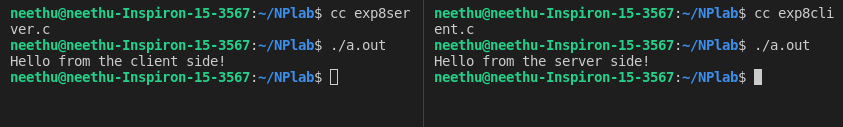
\includegraphics[scale=0.57]{img/e8.png}
\end{figure}

\subsection{Result}
Implemented the program for the Client-Server communication using Socket Programming and UDP as transport layer protocol using C language in Ubuntu 20.04 with kernel and the above outputs were obtained.

